\documentclass[11pt,a4paper]{article}
\usepackage[a4paper,margin=2.5cm]{geometry}
\setlength{\emergencystretch}{3em}
\usepackage{graphicx}
\usepackage{booktabs}
\usepackage{amsmath}
\usepackage{xcolor}
\usepackage{caption}
\usepackage[hidelinks]{hyperref}

\graphicspath{{figures/}}
\captionsetup{font=small,labelfont=bf}

\title{\textbf{Thread Scaling and SIMD Vectorisation for Dense Matrix
Multiplication:\\ A Controlled Benchmarking Study}}
\author{Alejandro Delgado Valera\\
\small BIG DATA -- Individual Assignment 3\\
\small Grado en Ciencia e Ingenier{\'i}a de Datos\\
\small Universidad de Las Palmas de Gran Canaria\\
\small \url{https://github.com/aledelgadoo/individual-assignments-bigdata}}
\date{October 27, 2026}

\begin{document}
\maketitle

\begin{abstract}
\noindent\textbf{Question:} how does the thread count $p$ affect the runtime of a
shared-memory dense matrix multiplication, when does parallel execution help, and
what does explicit SIMD vectorisation add once it is separated from thread-count
effects? The study compares an equivalent sequential baseline against an OpenMP
row-parallel implementation of the same validated \texttt{ikj} kernel
(\texttt{float64}, identical inputs, layout and arithmetic order), with the
parallel binary measured for $p \in \{1,2,4,8,12,16\}$ on a 10-core/12-thread
hybrid CPU (2 P-cores + 8 E-cores), plus a three-way vectorisation control
(scalar / compiler-default / \texttt{\#pragma omp simd}) at fixed $p$, and a
P-cores-only confinement run. Timings are medians of five batched repetitions of
the kernel; the sequential reference is bracketed around every thread sweep to
remove thermal drift. Speedup reaches $S(16)=2.59$ at $n=2000$
($E(16)=0.16$), efficiency peaks near $E(2)\approx0.8$ and collapses for small
$n$ where fork/join costs dominate ($T_p(1)/T_{seq}=1.26$ at $n=50$).
Oversubscribing the 12 hardware contexts with $p=16$ is neutral at large $n$
(within variability) and harmful at $n\le100$. Explicit vectorisation is worth
3.10$\times$ at $n=200$ down to 1.44$\times$ at $n=2000$ ($p=1$), and the
evidence shows GCC did \emph{not} vectorise the parallel loop by default, so the
pragma was necessary. Restricting execution to the four P-core threads is
12--14\,\% faster at $n=2000$. Claims are scoped to this kernel, machine and
protocol.
\end{abstract}

\section{Introduction and objective}

Assignments~1 and~2 established a validated single-threaded baseline: a dense
$O(n^3)$ multiplication whose \texttt{ikj} ordering is the fastest local variant
on this machine~\cite{strang2016,cormen2022}. This assignment asks how that
kernel behaves when it is executed by several hardware threads, and how much of
the observed behaviour is due to threads versus SIMD vectorisation.

\textbf{Research question.}
How does the thread count $p$ affect the multiplication time $T_p(n)$ of the
validated \texttt{ikj} kernel, for which tested sizes does parallel execution
beat the equivalent sequential baseline, and what speedup is attributable to
vectorisation when thread count is held fixed?

\textbf{Hypotheses (stated before measurement).}
\begin{enumerate}
  \item[H1:] Parallel speedup grows with $n$ and saturates well below $p$:
        fork/join overhead is large relative to small kernels, and at large $n$
        memory bandwidth and the heterogeneous P/E cores cap scaling.
  \item[H2:] The parallel implementation with one thread reveals framework
        overhead: $T_p(1) \ge T_{seq}(n)$, with the gap largest for small $n$.
  \item[H3:] Testing $p=16$ on 12 hardware execution contexts is an
        oversubscription configuration that brings no further gain and is most
        costly for small kernels.
  \item[H4:] At fixed $p$, the vectorised kernel is faster than the
        non-vectorised control, the gain shrinking as $n$ grows and the
        multiplication becomes memory-bound; compiler-default vectorisation of
        the parallel loop cannot be assumed and must be evidenced per binary.
\end{enumerate}

\section{Background}

\textbf{Speedup and efficiency.} With $T_{seq}(n)$ the sequential baseline time
and $T_p(n)$ the parallel time for the same input, $S(p)=T_{seq}(n)/T_p(n)$ and
$E(p)=S(p)/p \le 1$ for a workload that does not change~\cite{fleming1986,mytkowicz2009}.
Superlinear values ($S(p)>p$) would indicate a measurement or cache effect and
must be explained, not assumed~\cite{mytkowicz2009}.

\textbf{OpenMP.} A \texttt{parallel for} construct forks a team of $p$ threads,
executes the loop with a static partition over the outer index, and joins at an
implicit barrier~\cite{openmp}. Because the outer index selects a row of $C$,
each thread owns disjoint rows and the per-element summation order over $k$ is
unchanged, so results are bitwise identical for every $p$; the inner loop over
$j$ streams contiguous memory and is vectorisable.

\textbf{Hybrid CPUs.} The test machine pairs performance cores (P-cores,
SMT-scheduled as two logical CPUs each) with efficiency cores (E-cores, one
thread each). An equal static partition of rows gives every thread the same
\emph{number} of rows but not the same \emph{cost} per row, which limits $E(p)$
and makes thread placement part of the measurement~\cite{intelwapl}.

\textbf{SIMD.} With \texttt{-march=native} the compiler targets AVX2 with FMA
(32-byte vectors of four doubles; SSE4.2 and AVX enabled, AVX-512 disabled by
the toolchain on this CPU). Vectorisation can be requested explicitly with
\texttt{\#pragma omp simd}, and its effect must be separated from thread-count
effects by holding $p$ fixed~\cite{intelig}.

\section{Methodology}

\subsection{Implementations}

One C source (\texttt{src/kernels.c}) is compiled four ways; every binary runs
the same \texttt{ikj} kernel on the same \texttt{float64} row-major matrices and
differs only in the flags of Table~\ref{tab:builds}. The sequential baseline and
the parallel kernel perform the same operations in the same order (the parallel
loop only redistributes rows), so they are equivalent by construction; the only
documented differences are the OpenMP runtime linkage and the SIMD pragma.

\begin{table}[h!]
\centering
\small
\begin{tabular}{lll}
\toprule
Binary & Flags & Role \\
\midrule
\texttt{matmul3\_seq}    & \texttt{-O2 -march=native}                  & sequential baseline \\
\texttt{matmul3\_scalar} & \texttt{... -fopenmp -fno-tree-vectorize}   & parallel, no SIMD (control) \\
\texttt{matmul3\_auto}   & \texttt{... -fopenmp}                       & parallel, compiler default \\
\texttt{matmul3\_simd}   & \texttt{... -fopenmp -DUSE\_OMP\_SIMD}      & parallel, explicit pragma \\
\bottomrule
\end{tabular}
\caption{The four builds of one shared source (\texttt{-std=c11 -Wall
-Wextra}, link \texttt{-lpsapi -lm}). \texttt{simd} adds \texttt{\#pragma omp
simd} on the inner loop; all other code is identical.}
\label{tab:builds}
\end{table}

{\sloppy
Threading is controlled inside the process: \texttt{omp\_set\_dynamic(0)} plus
\texttt{omp\_set\_num\_threads($p$)} before every timed run fixes the team size
regardless of environment variables, and \texttt{schedule(static)} partitions
rows evenly. There is no BLAS or other library with internal threads, so the
reported $p$ is the whole configuration. Affinity is set at process level with
\texttt{Set\-Process\-AffinityMask}: \texttt{all} = CPU0--11 (default runs) and
\texttt{pcore} = CPU0--3 (the four P-core threads only); placement within the
mask is left to the Windows scheduler, as libgomp on Windows provides no
reliable binding---this is recorded as a limitation, not as a controlled
variable.\par}

\subsection{Inputs}

Dense $A_n, B_n$ for $n \in \{50,100,200,500,1000,2000\}$, generated as in
Assignments~1--2 (seed 42, uniform in $[-1,1]$, little-endian \texttt{<f8},
row-major) and reused byte for byte, so results are comparable with the earlier
reports. A third $n \times n$ buffer holds $C$, zeroed inside the timed kernel
(every multiplication is complete and independent).

\subsection{Correctness}

\texttt{selftest} (run on all four binaries, 31 checks for \texttt{seq}, 76 for
the parallel builds, 0 failures) verifies known products, zero and identity
matrices, random cases against a long-double reference ($\textit{rtol}=10^{-10}$,
$\textit{atol}=10^{-12}$) and, for the parallel builds, \textbf{bitwise
invariance} of the result for $p \in \{2,3,4,8,12\}$. During the campaign the
checksum of $C$ is emitted after every measured batch: across all 222 configs
and 1{,}110 measurements there is exactly one distinct checksum per $n$, i.e.
every variant, thread count and affinity produced bitwise-identical matrices.

\subsection{Environment}

Table~\ref{tab:env} summarises \texttt{data/results/environment.json}, captured
during the measurement session. The High-performance power plan was active for
the whole campaign and the Balanced plan restored afterwards.

\begin{table}[h!]
\centering
\small
\begin{tabular}{ll}
\toprule
Item & Value \\
\midrule
CPU & Intel Core i7-1355U hybrid: 2 P-cores (2 threads each, CPU0--3) \\
     & + 8 E-cores (1 thread each, CPU4--11); 10 physical, 12 logical CPUs \\
RAM / OS & 16.79 GB; Windows 10 (10.0.26200) \\
Compiler & GCC 16.1.0 (MinGW-w64 ucrt64); \texttt{-O2 -march=native} \\
Native ISA & AVX, AVX2, FMA, SSE4.2 enabled; AVX-512 disabled \\
OpenMP & GCC libgomp; team fixed per run; default active spin-waiting \\
Power plan & High performance (GUID \texttt{8c5e7fda-...}) during campaign \\
Python & 3.11.9, numpy 2.2.6, psutil 7.1.0 \\
\bottomrule
\end{tabular}
\caption{Execution environment. Clock read-outs from \texttt{psutil} were
unreliable on this platform (reported 1.7\,GHz flat) and are therefore not
quoted.}
\label{tab:env}
\end{table}

\subsection{Measurement protocol}

Each config (variant $\times$ $p$ $\times$ $n$ $\times$ affinity) follows the
common protocol of Assignment~2:
\begin{enumerate}
  \item \textbf{Probe:} one unchecked warm-up plus two timed single
        multiplications; a config is skipped if a probe exceeds the 60\,s
        budget; otherwise the bench budget is $\min(60\,\text{s}, 2\times
        \max(\text{probe, probe warm-up}))$---the warm-up term covers the cost
        of creating the thread team, which the first warm-up of the separate
        bench process pays again.
  \item \textbf{Bench:} one budget-checked warm-up, calibration by batch
        doubling until one batch lasts $\ge 0.2$\,s, then 5 measured
        repetitions of a full multiplication (kernel only: loads and checksums
        are outside the timed region; \texttt{memset} of $C$ is inside, as part
        of a complete multiplication).
  \item \textbf{Summary statistic:} the \textbf{median} of the 5 batched
        repetition times; variability is reported as the coefficient of
        variation (CV) across them. Memory is the peak resident set size of the
        process. Budgets: 60\,s and 4\,GiB per child; JSON lines of every run
        are kept in \texttt{data/results/raw\_detail/}.
\end{enumerate}

\textbf{Thermal bracketing (stability control).} A pilot campaign showed that
cross-phase comparisons were contaminated by clock drift on this laptop: the
same binary and config measured $3.22$\,s and $4.35$\,s ($+35$\,\%) in two
sessions, and $S(1)$ deviated to 0.66--0.76. The reported session therefore
(1) heat-soaks the machine for $\approx 2.5$\,min (two minutes of sustained
12-thread multiplications) until the package reaches steady state, and (2)
\emph{brackets} every thread sweep: for each $n$ the sequence is
\texttt{seqpre} $\rightarrow$ $p \in \{1,\dots,16\}$ $\rightarrow$
\texttt{seqpost}, with $T_{seq}(n)$ taken as the median of the 10 bracketed
sequential measurements taken seconds apart from the sweep. The \texttt{simd2}
and \texttt{pcore2} blocks run back-to-back in the same session. All 96
stable-session configs and all 126 earlier configs finished with status
\texttt{ok}; the earlier (drifted) rows are retained in the CSVs for
transparency but the report quotes the stable session only.

\section{Results}

\subsection{Runtime, speedup and efficiency}

Table~\ref{tab:runtime} gives the medians behind every $S$ and $E$;
Table~\ref{tab:scaling} collects $S(p)$ and $E(p)$. Median CV across the 36
scaling configs is 5.1\,\% (max 13.6\,\%). Figures~\ref{fig:runtime}
to~\ref{fig:efficiency} show the same data graphically.

\begin{table}[h!]
\centering
\small
\setlength{\tabcolsep}{4pt}
\begin{tabular}{r|rrrrrrr}
\toprule
 &  & \multicolumn{6}{c}{parallel time $T_p(n)$ (ms)} \\
$n$ & $T_{seq}$ (ms) & $p{=}1$ & $p{=}2$ & $p{=}4$ & $p{=}8$ & $p{=}12$ & $p{=}16$ \\
\midrule
50   & 0.018   & 0.022   & 0.045   & 0.057   & 0.089   & 0.097   & 0.124 \\
100  & 0.159   & 0.173   & 0.160   & 0.160   & 0.160   & 0.216   & 0.194 \\
200  & 1.408   & 1.313   & 0.917   & 0.790   & 0.653   & 0.660   & 0.648 \\
500  & 21.488  & 21.982  & 14.267  & 12.701  & 10.841  & 10.410  & 10.117 \\
1000 & 233.654 & 235.686 & 167.644 & 124.109 & 119.753 & 91.202  & 92.933 \\
2000 & 3626.93 & 3906.35 & 2646.38 & 1916.77 & 1490.82 & 1412.58 & 1398.74 \\
\bottomrule
\end{tabular}
\caption{Median kernel time per multiplication (ms), median of five batched
repetitions; $T_{seq}$ = median of the 10 bracketed sequential runs.}
\label{tab:runtime}
\end{table}

\begin{table}[h!]
\centering
\small
\setlength{\tabcolsep}{5pt}
\begin{tabular}{r|rrrrrr}
\toprule
$n$ & $p{=}1$ & $p{=}2$ & $p{=}4$ & $p{=}8$ & $p{=}12$ & $p{=}16$ \\
\midrule
50   & 0.79\,(0.79) & 0.39\,(0.20) & 0.31\,(0.08) & 0.20\,(0.03) & 0.18\,(0.02) & 0.14\,(0.01) \\
100  & 0.92\,(0.92) & 1.00\,(0.50) & 1.00\,(0.25) & 1.00\,(0.13) & 0.74\,(0.06) & 0.82\,(0.05) \\
200  & 1.07\,(1.07) & 1.54\,(0.77) & 1.78\,(0.45) & 2.16\,(0.27) & 2.13\,(0.18) & 2.17\,(0.14) \\
500  & 0.98\,(0.98) & 1.51\,(0.75) & 1.69\,(0.42) & 1.98\,(0.25) & 2.06\,(0.17) & 2.12\,(0.13) \\
1000 & 0.99\,(0.99) & 1.39\,(0.70) & 1.88\,(0.47) & 1.95\,(0.24) & 2.56\,(0.21) & 2.51\,(0.16) \\
2000 & 0.93\,(0.93) & 1.37\,(0.69) & 1.89\,(0.47) & 2.43\,(0.30) & 2.57\,(0.21) & 2.59\,(0.16) \\
\bottomrule
\end{tabular}
\caption{Speedup $S(p)$ with efficiency $E(p)$ in parentheses.}
\label{tab:scaling}
\end{table}

\begin{figure}[h!]
\centering
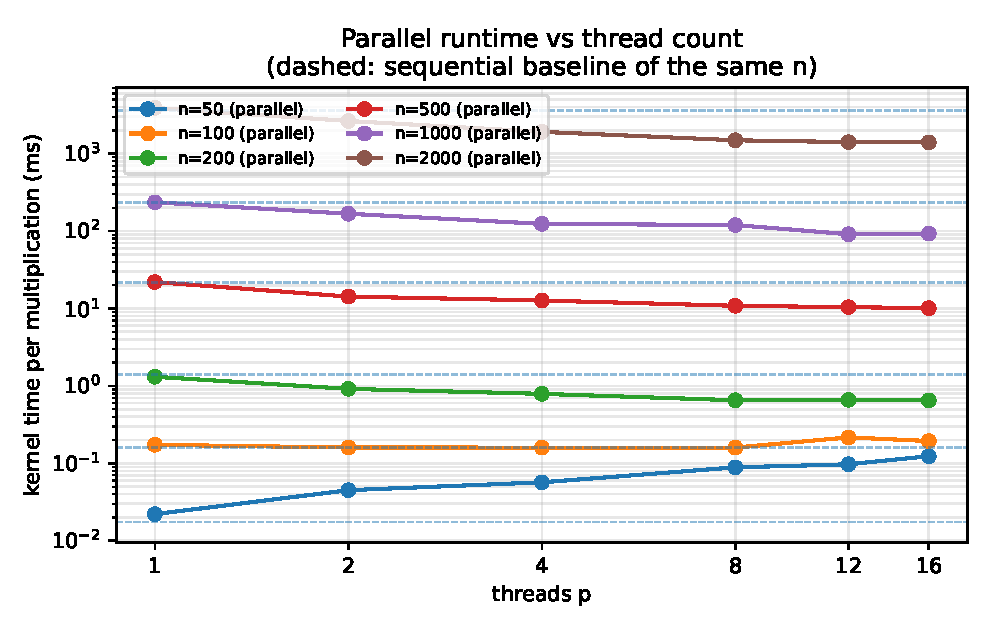
\includegraphics[width=0.82\textwidth]{fig1_runtime.pdf}
\caption{Kernel time vs thread count (log scale); dashed lines are the
bracketed sequential baselines.}
\label{fig:runtime}
\end{figure}

\begin{figure}[h!]
\centering
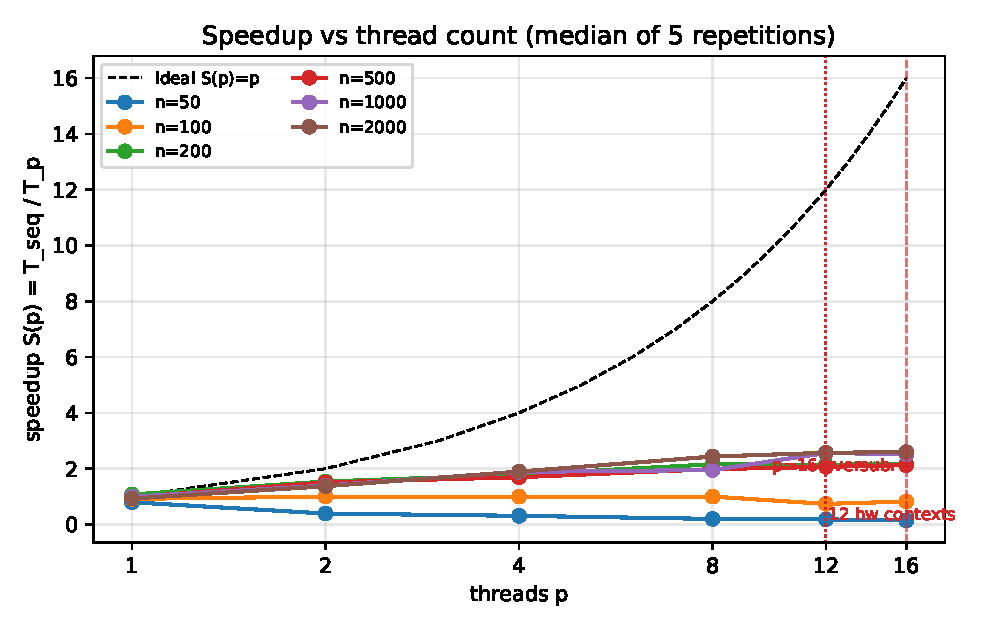
\includegraphics[width=0.82\textwidth]{fig2_speedup.pdf}
\caption{Speedup vs thread count against the ideal $S(p)=p$. The dotted line
marks the 12 hardware contexts, the dashed line the oversubscribed $p=16$.}
\label{fig:speedup}
\end{figure}

\begin{figure}[h!]
\centering
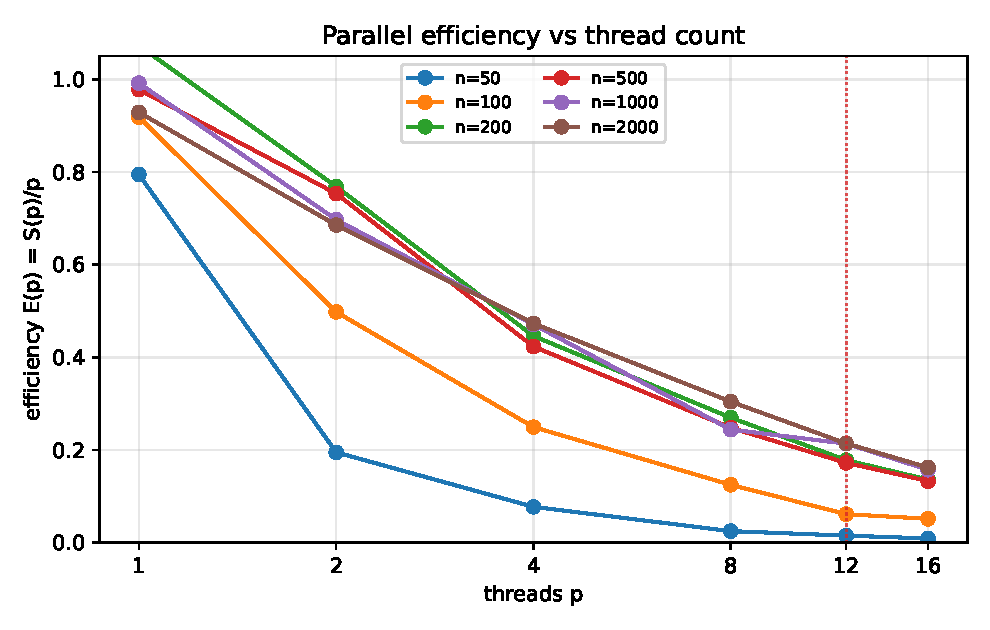
\includegraphics[width=0.82\textwidth]{fig3_efficiency.pdf}
\caption{Efficiency vs thread count.}
\label{fig:efficiency}
\end{figure}

\textbf{When does parallelism help?} Only for $n \ge 200$: at $n=50$
$T_p(p)>T_{seq}$ for every $p$, and at $n=100$ the parallel time is flat at
$\approx0.16$\,ms for $p \le 8$, i.e.\ the fixed cost of the parallel region
($\sim$15--30\,$\mu$s per multiplication at this size) dominates and extra
threads do not shorten it. For $n \ge 200$ the sweep is monotone up to $p=8$
and saturates: the best observed speedups are $S(12)=2.56$ at $n=1000$ and
$S(16)=2.59$ at $n=2000$, with $E \le 0.77$ everywhere (best at $p=2$ for
$n \ge 200$). No configuration is superlinear; the only point above parity at
$p{=}1$ is $S(1)=1.07$ at $n=200$, which is within that config's 8.2\,\% CV and
is not claimed as a real gain.

\subsection{Framework overhead with one thread}

\begin{table}[h!]
\centering
\small
\begin{tabular}{rrrr}
\toprule
$n$ & $T_{seq}$ ($\mu$s) & $T_p(1)$ ($\mu$s) & $T_p(1)/T_{seq}$ \\
\midrule
50   & 17.52    & 22.05    & 1.26 \\
100  & 159.27   & 173.49   & 1.09 \\
200  & 1408.39  & 1313.17  & 0.93 \\
500  & 21488.46 & 21981.88 & 1.02 \\
1000 & 233653.80 & 235686.20 & 1.01 \\
2000 & 3626931.85 & 3906349.60 & 1.08 \\
\bottomrule
\end{tabular}
\caption{Parallel implementation with one thread vs the sequential baseline
(hypothesis H2).}
\label{tab:overhead}
\end{table}

Table~\ref{tab:overhead} confirms H2 in the regime where it matters: at
$n=50$ the single-threaded parallel run is 26\,\% slower---about
4.5\,$\mu$s of fork/join on an 17.5\,$\mu$s kernel. For $n \ge 200$ the ratio
stays within $\pm 8$\,\% of parity (both binaries run the same vectorised
inner loop), with the $+8$\,\% at $n=2000$ attributable to residual
within-session drift between the bracketed baseline and the sweep start.

\subsection{Vectorisation (optional extension)}

Thread count is held fixed while only the build changes (the \texttt{simd2}
block, all three variants measured back-to-back). Evidence that vectorisation
occurs: \texttt{-fopt-info-vec-optimized} reports the inner loop of
\texttt{matmul3\_seq} and of the pragma build vectorised with 32-byte vectors,
and per-symbol \texttt{objdump} finds packed FMA arithmetic in
\texttt{matmul\_ikj\_seq} (2) and in \texttt{matmul\_ikj\_par.\_omp\_fn.0}
(2) of the \texttt{simd} binary, while the \texttt{scalar} binary contains
none (0). The same inspection of \texttt{matmul3\_auto} shows packed
instructions only in the sequential function it never calls: \textbf{GCC did not
vectorise the outlined parallel loop under \texttt{-O2}, so the explicit pragma
was necessary} (hypothesis H4's caution). Full listings are in
\texttt{data/results/vectorisation.txt}.

\begin{table}[h!]
\centering
\small
\begin{tabular}{rrrrrrr}
\toprule
 & \multicolumn{3}{c}{time at $p=1$ (ms)} & \multicolumn{3}{c}{scalar/simd gain} \\
$n$ & scalar & auto & simd & $p{=}1$ & auto/simd & $p{=}8$ \\
\midrule
200  & 3.46    & 3.47    & 1.12    & 3.10 & 3.11 & 1.79 \\
500  & 60.80   & 50.79   & 24.54   & 2.48 & 2.07 & 1.83 \\
1000 & 506.99  & 502.37  & 254.34  & 1.99 & 1.98 & 1.64 \\
2000 & 5080.69 & 5205.41 & 3538.06 & 1.44 & 1.47 & 1.47 \\
\bottomrule
\end{tabular}
\caption{Vectorisation control at fixed thread count (\texttt{simd2} block).
\texttt{auto} tracks \texttt{scalar} because the parallel loop was not
vectorised by default.}
\label{tab:simd}
\end{table}

\begin{figure}[h!]
\centering
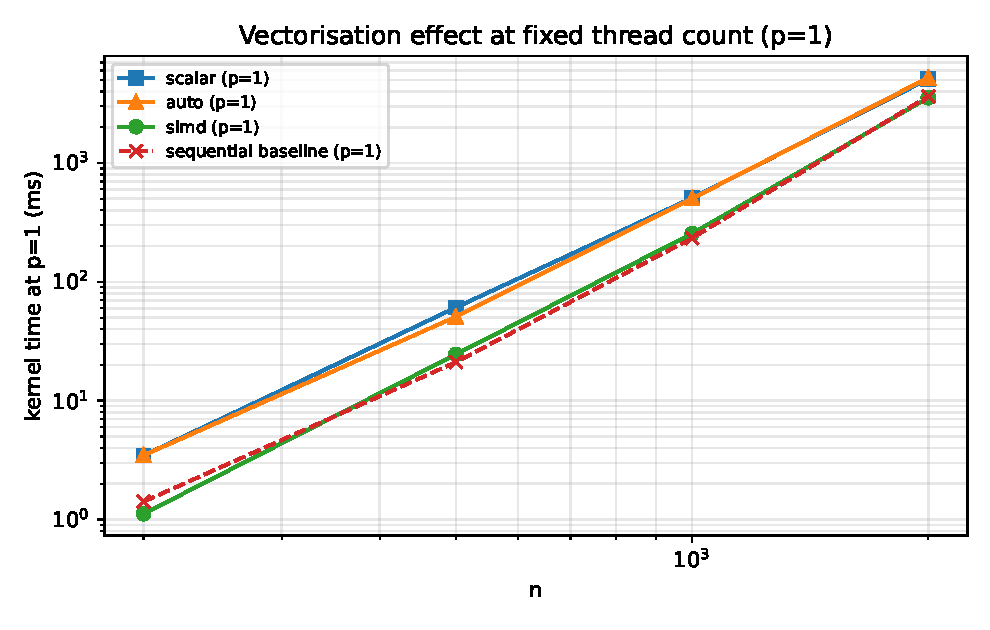
\includegraphics[width=0.82\textwidth]{fig4_simd.pdf}
\caption{Vectorisation effect at $p=1$; the sequential baseline uses the same
vectorised inner loop as \texttt{simd}.}
\label{fig:simd}
\end{figure}

Table~\ref{tab:simd} and Figure~\ref{fig:simd} quantify H4: the pragma is
worth 3.10$\times$ at $n=200$ but only 1.44$\times$ at $n=2000$ ($p=1$),
because at $n=200$ the working set fits in cache (compute-bound, close to the
4$\times$ width of 256-bit vectors over scalar), while at $n=2000$ the three
32\,MB matrices stream from DRAM and the arithmetic is no longer the
bottleneck. The gain persists at high thread counts (1.47--1.83$\times$ at
$p=8$): vectorisation and threading compose, and their effects are separated by
construction---all rows of Table~\ref{tab:scaling} use one binary
(\texttt{simd}), while Table~\ref{tab:simd} varies only the binary at fixed
$p$. The scalar column additionally bounds the ``compiler default''
configuration, whose parallel loop is scalar as shown above.

\subsection{Oversubscription at $p=16$}

The hardware provides 12 execution contexts, so $p=16$ is an oversubscribed
configuration (H3). Observed effect (Tables~\ref{tab:runtime}
and~\ref{tab:scaling}): at $n=2000$, $p=16$ is within CV of $p=12$
($S$: 2.59 vs.\ 2.57, i.e.\ $+0.8$\,\%, below the 3.7--3.9\,\% CV of those
configs)---no gain, no collapse; at $n=1000$ it is 2\,\% slower; at $n=100$
it is 10\,\% slower than $p=12$ and at $n=50$ 28\,\% slower, because sixteen
thread wake-ups and barrier crossings are paid for a kernel that is shorter
than the parallel region itself. Efficiency at $p=16$ never exceeds 0.16.
Oversubscription is therefore confirmed as \emph{pointless}: the extra runnable
threads only contend for the same 12 contexts while adding scheduling and
barrier cost that shows up exactly where the useful work is smallest.

\subsection{P-cores vs.\ all cores}

\begin{table}[h!]
\centering
\small
\begin{tabular}{rrrrr}
\toprule
$n$ & $p$ & all CPUs (ms) & P-cores only (ms) & ratio \\
\midrule
500  & 1 & 21.98  & 22.05  & 1.00 \\
500  & 2 & 14.27  & 15.46  & 1.08 \\
500  & 4 & 12.70  & 13.72  & 1.08 \\
1000 & 1 & 235.69 & 266.62 & 1.13 \\
1000 & 2 & 167.64 & 165.37 & 0.99 \\
1000 & 4 & 124.11 & 113.19 & 0.91 \\
2000 & 1 & 3906.35 & 3443.15 & 0.88 \\
2000 & 2 & 2646.38 & 2280.18 & 0.86 \\
2000 & 4 & 1916.77 & 1755.45 & 0.92 \\
\bottomrule
\end{tabular}
\caption{Same binary and $p$ with the process confined to CPU0--3 (P-core
threads) vs.\ CPU0--11 (ratio $<$ 1 favours the P-cores-only run).}
\label{tab:pcore}
\end{table}

\begin{figure}[h!]
\centering
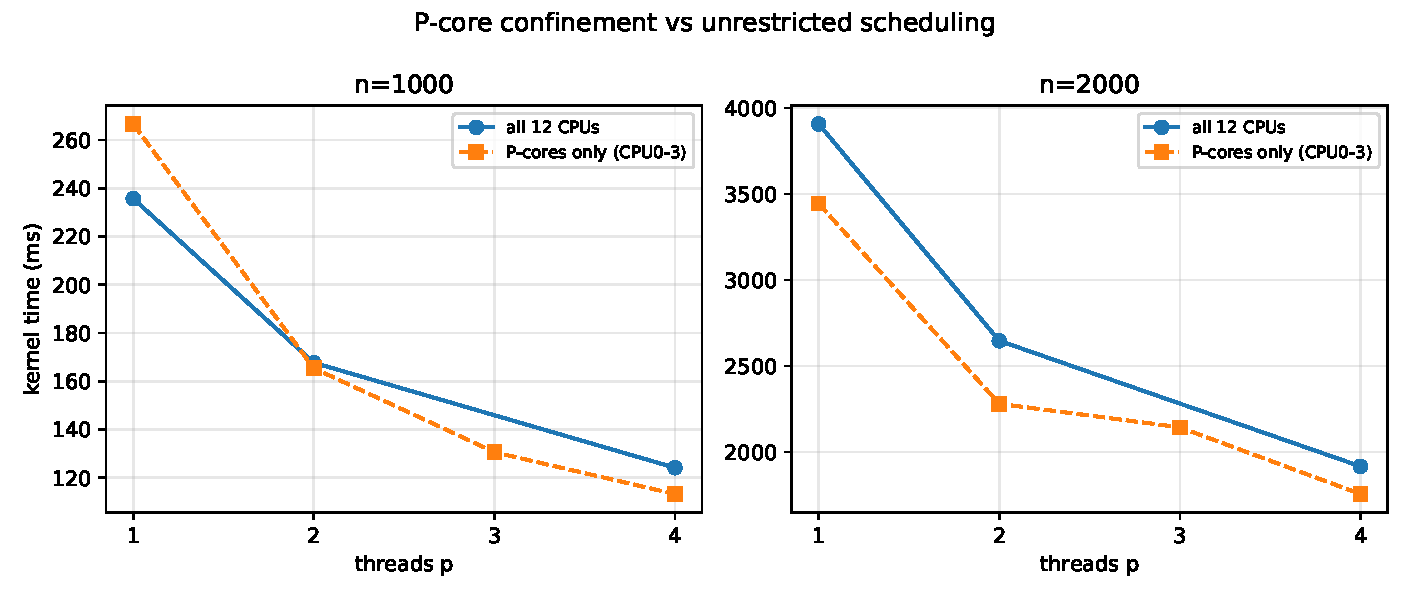
\includegraphics[width=0.95\textwidth]{fig5_pcore.pdf}
\caption{P-core confinement vs.\ unrestricted scheduling.}
\label{fig:pcore}
\end{figure}

At $n=2000$ (Table~\ref{tab:pcore}, Figure~\ref{fig:pcore}) confining to the
four P-core threads is 12--14\,\% faster than allowing the OS to schedule over
all 12 contexts: the P-cores do more work per cycle and no E-core thread
becomes the slowest partition behind the barrier. At $n=1000$ the effect
changes sign with $p$ and at $n=500$ the restricted run is 8\,\% slower---all
within the $\pm 13$\,\% variability band of these medium configs---so the
confinement advantage is a large-$n$ result only.

\subsection{Memory}

Peak resident memory (all configs of a given $n$) is 5.4, 6.2, 11.0, 28.2 and
96.8\,MB for $n=50,200,500,1000,2000$ respectively; at $n=2000$ that is
essentially $3 \times 32$\,MB of matrices plus process overhead, identical for
every $p$: static row partitioning allocates no per-thread copies and creates
no shared-data races (consistent with the bitwise checksum invariance).

\section{Discussion}

\textbf{Answer to the research question.} On this machine and kernel,
parallel execution helps only from $n=200$ upwards and only up to about
$p=8$--$12$: the measured ceiling is $S \approx 2.6$, far below $p=12$. The
evidence attributes this to three compounding effects: (1) fixed parallel-region
costs, which are 26\,\% of a $n=50$ multiplication and explain the flat
$n=100$ curve; (2) heterogeneity---an equal row partition is not equal work on
2 P-cores + 8 E-cores, and the P-cores-only run beating the all-CPU run by up
to 14\,\% at $n=2000$ shows placement matters at large $n$; and (3)
memory---at $n=2000$ the streaming of three 32\,MB matrices bounds the useful
parallelism, which also caps the vectorisation gain at 1.44$\times$. H1, H2,
H3 and H4 are all supported by the data above, with H4's second part (default
vectorisation cannot be assumed) demonstrated per binary rather than assumed.

\textbf{Methodological findings.} Two instrument bugs were found and fixed
before the reported session: a gate that ignored the thread-team creation cost
of the bench process (fixed by including the probe warm-up in the gate), and
cross-phase thermal drift that depressed $S(1)$ to 0.66 (fixed by heat-soak and
sequential bracketing). The pilot rows are kept in the CSVs; the stability of
the reported session is visible as $S(1) \in [0.92, 1.07]$ for $n \ge 100$ and
median CV 5.1\,\%.

\textbf{Limitations.}
\begin{itemize}
  \item One hybrid laptop, one kernel, one input distribution; results do not
        generalise to servers, other BLAS libraries or structured data.
  \item Windows schedules threads inside the affinity mask; P/E placement and
        boost states were not pinned per thread, so $\pm 5$--13\,\% run-to-run
        variability remains (median CV 5.1\,\%).
  \item The sequential baseline and the parallel binary differ in linkage and
        in the OpenMP region by construction; at $p=1$ a residual $\pm 8$\,\%
        gap remains (drift, scheduling), so $S(1)$ is parity within noise, not
        an exact 1.00.
  \item Efficiency losses are not decomposed into bandwidth counters
        (no hardware counters were collected on Windows).
  \item The \texttt{auto} build's missing vectorisation is a GCC 16
        \texttt{-O2} cost-model outcome; other compilers or \texttt{-O3} may
        differ.
\end{itemize}

Following the assignment guidance, claims are limited to these
implementations, inputs and hardware~\cite{fleming1986,mytkowicz2009}.

\section{Conclusions}

Within the tested scope: (1) the OpenMP row-parallel \texttt{ikj} kernel beats
its equivalent sequential baseline only for $n \ge 200$, peaking at
$S(12)=2.56$ ($n=1000$) and $S(16)=2.59$ ($n=2000$), i.e.\ threads buy $\le
2.6\times$ on 12 hardware contexts; (2) efficiency is the binding metric:
$E(p) \le 0.77$ everywhere and $\le 0.21$ for $p \ge 12$, driven by fixed
parallel-region cost at small $n$ and by P/E asymmetry plus memory bandwidth at
large $n$; (3) one-thread parallel overhead is 26\,\% at $n=50$ and within
$\pm 8$\,\% of parity for $n \ge 200$; (4) oversubscribing ($p=16>12$) yields
no gain at large $n$ and up to $-28$\,\% at $n=50$, confirming it is
harmful exactly where the per-thread work is least; (5) explicit
\texttt{\#pragma omp simd} is worth 1.4--3.1$\times$ at fixed thread count,
was \emph{necessary} because GCC's default did not vectorise the parallel loop,
and composes with threading; and (6) confining the process to the four P-core
threads is 12--14\,\% faster at $n=2000$.

Unresolved: whether the scaling ceiling moves if rows are weighted by core
type, whether bandwidth can be relieved by tiling in the parallel kernel, and
how these results compare with a distributed implementation
(Assignment~4).

\section{References and materials}

{\sloppy
All source code, shared inputs, raw measurements (CSV per config and JSON lines
per run), \texttt{environment.json}, \texttt{vectorisation.txt}, the executed
analysis notebook and every figure live in the public repository
\url{https://github.com/aledelgadoo/individual-assignments-bigdata}. The Git
tag \texttt{assignment-3} marks the exact submitted state (tags
\texttt{assignment-1} and \texttt{assignment-2} preserve the earlier reports).
\texttt{README.md} documents the build, input-generation, self-test,
campaign and analysis commands that regenerate this report end to end; the
notebook \texttt{notebooks/03\_analysis.ipynb} writes the summary tables
(\texttt{summary\_scale.csv}, \texttt{summary\_simd.csv},
\texttt{summary\_pcore.csv}) quoted here.\par}

\section*{Generative-AI usage statement}

Following the course policy, the author discloses that the AI assistant
\textbf{opencode} (model \texttt{opencode/mimo-v2.6-flash-free}) was used, under
the author's direction, for planning the OpenMP/SIMD design and the
measurement protocol, drafting and debugging the C code and Python scripts,
diagnosing the two pilot-campaign instrument bugs, generating the analysis
notebook and figures, and revising the English of this report. The author
reviewed all generated code, ran and inspected the self-tests, supervised every
campaign execution, verified the numbers quoted here against the raw CSV files,
and is responsible for the measurements, the conclusions and any errors.

\begin{thebibliography}{9}
\bibitem{strang2016}
G. Strang, \emph{Introduction to Linear Algebra}, 5th ed.
Wellesley--Cambridge Press, 2016.

\bibitem{cormen2022}
T. H. Cormen, C. E. Leiserson, R. L. Rivest, and C. Stein,
\emph{Introduction to Algorithms}, 4th ed. MIT Press, 2022.

\bibitem{openmp}
OpenMP Architecture Review Board, \emph{OpenMP Specification for Offload and
Shared Memory, Version 5.2}, 2022. [Online]. Available:
\url{https://www.openmp.org/specifications/}

\bibitem{intelwapl}
Intel Corporation, \emph{Intel Hyper-Threading Technology: Software
Optimization Guide} and Alder Lake performance/efficiency-core
documentation. [Online]. Available: \url{https://www.intel.com/}

\bibitem{intelig}
Intel Corporation, \emph{Intel Intrinsics Guide} (AVX2/FMA instruction
reference). [Online]. Available: \url{https://www.intel.com/}

\bibitem{fleming1986}
W. P. Fleming and J. M. Wallace, ``How not to lie with statistics: the correct
way to summarize benchmark results,'' \emph{Communications of the ACM},
vol. 29, no. 3, pp. 218--221, 1986.

\bibitem{mytkowicz2009}
T. Mytkowicz, A. Diwan, M. W. Hauswirth, and P. F. Sweeney,
\emph{Measuring Computer Performance: A Practitioner's Guide}.
Cambridge University Press, 2009.

\bibitem{isoC11}
ISO/IEC 9899:2011, ``Information technology --- Programming languages --- C,''
International Organization for Standardization, 2011.

\bibitem{psutil}
G. Rodola, \emph{psutil: cross-platform process and system utilities}, 2026.
[Online]. Available: \url{https://github.com/giampaolo/psutil}
\end{thebibliography}

\end{document}
